\def\lncs{1}

\documentclass[]{article}
\RequirePackage{amsmath}

\usepackage{graphicx}
\usepackage{amssymb}
\usepackage{color}
\usepackage{hyperref}
\usepackage{float}
\usepackage{algorithm}
\usepackage{algpseudocode}

\bibliographystyle{IEEEtran}

\newcommand{\knote}[1]{{\textcolor{green}{Alex notes:{#1}}}}
\newcommand{\dnote}[1]{{\textcolor{red}{DNotes:{#1}}}}
\newcommand{\snote}[1]{{\textcolor{blue}{SNotes:{#1}}}}

\newcommand{\Ergo}{Ergo}
\newcommand{\Erg}{Erg}
\newcommand{\nanoErg}{nanoErg}
\def\Let#1#2{\State #1 $:=$ #2}
\def\LetRnd#1#2{\State #1 $\gets$ #2}

\begin{document}
    \title{Ergo: A Resilient Platform For Contractual Money}
    \author{Ergo Developers, https://ergoplatform.org}
    \date{May 14, 2019\\v1.0}

    \maketitle

    \begin{abstract}
        We present Ergo, a new flexible blockchain protocol.
        Ergo is designed for developing decentralized applications with the main focus of providing an efficient, secure and easy way to implement financial contracts.

        To achieve this goal, Ergo includes various technical and economic improvements to existing
        blockchain solutions. Every coin in Ergo is protected by a program in ErgoScript, which is
        a powerful and protocol-friendly scripting language based on $\Sigma$-protocols.
        Using ErgoScript, we can encode the conditions under which coins may be used: who can spend them,
        when, under what external conditions, to whom, and so on.

        Extended support for light nodes makes Ergo friendly for end users because it allows running 
        contracts on untrusted commodity hardware.
        To be usable in the long-term, Ergo follows a survivability approach -- it uses
        widely-researched solutions that don't result in security issues in the future,
        while also preventing performance degradation over time with the new economic model.
        Finally, Ergo has a self-amendable protocol that allows it to absorb new ideas and
        improve itself in the future.
\end{abstract}

    \section{Introduction}
\label{sec:intro}

% say the WHY creating Ergo. And also attack the existing financial system a few times.
% Important the readers know that Ergo really is in the same spirit of Bitcoin in the sense it is open,
% permissionless and is designed to disintermediate trusted third parties. But then we need to make clear if
% not too directly that Bitcoin/Ethereum still face a lot of challenges that Ergo is built to address.

Started more than ten years ago with Bitcoin~\cite{nakamoto2008bitcoin}, blockchain technology has so far proved
to be a secure way of maintaining a public transaction ledger and disintermediating trusted third parties such as 
traditional financial institutions to some degree.
Even after achieving a market capitalization over \$300bn in 2017~\cite{btcPrice},
no severe attacks were performed on the Bitcoin network despite the high potential yield.
This resilience of cryptocurrencies and the financial empowerment and self-sovereignty they promise to bring is
achieved by a combination of modern cryptographic algorithms and decentralized architecture.

However, this resilience comes at a cost 
%does not come for free 
and has not yet been proven for existing systems in the long-run at economy-wide scale.
To use a blockchain without any trust, its participants should check each other by downloading and
processing all the transactions in the network, utilizing network resources.
Besides network utilization, transaction processing also utilizes computational resources,
especially if the transactional language is flexible enough.
Finally, blockchain participants have to keep quite a significant amount of data in their local storages and
the storage requirements are growing fast. Of this, certain data must be maintained in memory.
Thus, transaction processing utilizes various resources of hundreds of thousands of computers all over the world
and consumption of these resources is paid for by regular users in the form of transaction fees~\cite{chepurnoy2018systematic}.
Despite the generous block reward subsidy in some existing systems, their fees is still very high~\cite{bitcoinFees}. Due to this, despite being around for more than ten years, blockchain technology is still primarily being used in financial applications, where the advantage of high security outweighs the disadvantage of high transaction costs.

Besides the vanilla currency example, the other use of blockchains is to build decentralized applications.
Such applications utilize the ability of the underlying platform to write smart contracts~\cite{szabo1994smart} implementing their logic by means of a blockchain-specific programming language.
One way to classify blockchains in terms of their ability to write smart contracts is based on if they are  
{\em UTXO-based}~(e.g., Bitcoin) or {\em account-based}~(e.g., Ethereum)~\cite{zahnentferner2018chimeric}. 
Account-based cryptocurrencies, such as Ethereum, introduce special contract accounts controlled by code,
that may be invoked by incoming transactions.
Although this approach allows performing arbitrary computation, the implementation of complex spending conditions
can lead to bugs such as the one in an Ethereum's `simple' multi-signature contract that caused a loss of \$150 million in 2017~\cite{parityLock}.
In UTXO-based cryptocurrencies, every coin has a script associated with it, and to spend that coin, one must satisfy the conditions given in the script. 
Implementing such protecting conditions is much easier with the UTXO model but doing arbitrary Turing-complete computation is quite complex~\cite{chepurnoy2018self}. However, most financial contracts do not require Turing-completeness. Ergo is based on the UTXO model and provides a convenient way to implement financial applications covering an
overwhelming majority of public blockchain use-cases.

While the contractual component is important for building decentralized applications,
it is also essential that the blockchain survives in the long-term.
Application-oriented blockchain platforms have existed only for a few years and the whole area is quite young. Since such platforms have already encountered problems with performance degradation over time~\cite{???}, their long-term survivability is questionable.
Even older UTXO-based money-oriented blockchains have not been proven to be fully resilient in the long-run
under changing conditions because we only have about 10 years of blockchain history up to this point.
Solutions for long-term survivability include concepts 
such as light nodes with minimal storage requirements~\cite{reyzin2017improving},
storage-rent fee component to prevent bloating of full-nodes~\cite{chepurnoy2018systematic}, and 
self-amendable protocols that can adapt to the changing environment and improve themselves without
trusted parties~\cite{goodman2014tezos}.
What is needed is a combination of various scientific ideas together to fix these problems, while also
providing a way for further improvements without any breaking changes and this is exactly what Ergo seeks to accomplish.



    \section{\Ergo{} philosophy}
\label{sec:social}

\knote{Ergo Vision And The Social Contract ?}

\Ergo{} protocol is very flexible and may be changed in the future by the community.
In this section we define the main principles, that should be followed during the \Ergo{} live.
In case of intentional violation of any of these principles, the resulting protocol should not
be called \Ergo{}.

\begin{itemize}
    \item{\em Decentralization first.} \Ergo{} should be as decentralized as possible: any parties (social leaders, software developers, hardware manufacturers, miners, funds and so on)
    which absence or malicious behavior may affect the security of the network should be avoided.
    If any of these parties will appear during \Ergo{} live, the community should consider ways how to decrease their impact level.
    \item{\em Created for regular people.} \Ergo{} is the platform for ordinary people, and their interests should not be infringed upon in favor of big parties.
    In particular, that means that regular people should be able to participate in the protocol by running a full node and mining blocks (albeit with a small probability).
    \item{\em Platform for Contractual money.} \Ergo{} is the base layer to applications, that will be built on top of it.
    It is suitable for any applications, but the main focus is to provide an efficient, secure and easy way to implement financial contracts.
    \item{\em Long terms focus.} All aspects of \Ergo{} development should be focused on a long-term perspective.
    At any point of time, \Ergo{} should be able to survive for centuries without expected hard forks,
    software or hardware improvements or some other unpredictable changes. As far as \Ergo{} is oriented to be a platform, applications built on top of \Ergo{} should also be able to survive in the long term.
    \item{\em Permissionless and open.} \Ergo{} protocol does not restrict or limit any categories of usage.
    It should allow anyone to join the network and participate in the protocol without any preliminary actions.
    No bailouts, blacklists or other forms of discrimination should be possible on the core level of \Ergo{} protocol.
    On the other hand application developers are free to implement any logic they want, taking responsibility for the ethics and legality of their application.
\end{itemize}

    \section{Autolykos Consensus Protocol}
\label{sec:autolykos}

% Почему выбрали PoW
% Известные проблемы PoW
% Детали Автоликуса

The core component of any blockchain system is its consensus protocol.
Despite extensive research of possible alternatives to the original Proof-of-Work (PoW) protocol
with the longest chain rule,
is still in demand due to simplicity, high-security guarantees, and friendliness to light clients.
However, a decade of extensive testing revealed several problems of the original one-CPU-one-vote idea.

First known problem of PoW is that development of specialized hardware (ASIC) allows
a small group of ASIC-equipped miners to solve PoW puzzles orders of magnitude faster and more efficiently
than everyone else. This problem can be solved with the help of memory-hard PoW schemes,
that reduce the disparity between the ASICs and commodity hardware. The most promising approach here
is to use asymmetric memory-hard PoW schemes that require significantly less memory
to verify a solution than to find it~\cite{biryukov2017equihash,ethHash}.

The second known threat to a PoW network decentralization is that even big miners trend to unite in
mining pools, leading to a situation when just a few pool operators (5 in Bitcoin, 2 in Ethereum
at the time of writing) control more than 51\% of computational power.
Although the problem has already been discussed in the community, no practical solutions were
implementer before \Ergo{}.


Ergo PoW protocol, Autolykos~\cite{Ergopow}, is the first consensus protocol, that is both memory-hard
and pool-resistant.
Autolykos is based on one list $k$-sum problem: miner should find
$k=32$ elements from the pre-defined list $R$ of size $N=2^{26}$~(which have a size of 2 Gb),
such that $\sum_{j \in J} r_{j} - sk = d$ is in the interval $\{-b,\dots,0,\dots,b\mod q\}$.
Elements of list $R$ are obtained as a result of one-way computation from index $i$,
two miner public keys $pk,w$ and hash of block header $m$ as $r_i=H(i||M||pk||m||w)$,
where $H$ is a hash function which returns the values in $\mathbb{Z}/q\mathbb{Z}$ and
$M$ is a static big message that is used to make hash calculation slower.
Also, we require a set of element indexes $J$ to be obtained
by one-way pseudo-random function $genIndexes$, that prevents possible solutions
search optimizations.

Thus we assume that the only option for a miner is to use the simple brute-force algorithm~\ref{alg:prove} to
create a valid block.

\begin{algorithm}[H]
    \caption{Block mining}
    \label{alg:prove}
    \begin{algorithmic}[1]
        \State \textbf{Input}: upcoming block header hash $m$, key pair $pk=g^{sk}$
        \State Generate randomly a new key pair $w=g^x$
        \State Calculate $r_{i \in [0,N)}=H(j||M||pk||m||w)$
        \While{$true$}
        \LetRnd{$nonce$}{$\mathsf{rand}$}
        \Let{$J$}{$genIndexes(m||nonce)$}
        \Let{$d$}{$\sum_{j \in J}{r_j} \cdot x - sk \mod q$}
        \If{$d < b$}
        \State \Return $(m,pk,w,nonce,d)$
        \EndIf
        \EndWhile
    \end{algorithmic}
\end{algorithm}

\knote{no genIndexes details}
\dnote{do you think we need full details in whitepaper? We've written that $genIndexes$ is "one-way pseudo-random function",
I think it is enough to catch the general idea}

Note that although the mining process utilizes private keys, the solution itself
only contains public keys. Solution verification can be performed by Alg.~\ref{alg:verify}.

\begin{algorithm}[H]
    \caption{Solution verification}
    \label{alg:verify}
    \begin{algorithmic}[1]
        \State \textbf{Input}: $m,pk,w,nonce,d$
        \State require $d < b$
        \State require $pk,w\in \mathbb{G}$ and $pk,w \ne e$
        \Let{$J$}{$genIndexes(m||nonce)$}
        \Let{$f$}{$\sum_{j \in J} H(j||M||pk||m||w)$}
        \State require $w^f = g^d \cdot pk$
    \end{algorithmic}
\end{algorithm}

This approach prevents mining pool formation, as soon as a miner that found a correct solution
can always try to steal the block reward as far as he knows the secret key $sk$. On the other hand,
it is secure to reveal a single solution, as soon as it only operates with public keys and reveals only one
linear relation between 2 secrets $sk, w$.

Memory-hardness follows from the fact that Algorithm~\ref{alg:prove} requires to keep
the whole list $R$ during the main loop execution.
Every list element takes 32 bytes, so the whole list of $N$ elements
takes $N \cdot 32 = 2 Gb$ of memory.
Miner can try to reduce memory requirements by calculating these elements ``on fly''
without keeping them in memory, however, in such a case he'll need to calculate the same
hash $H$ multiple~(for about $10^4$ for modern GPUs) times, reducing miner's efficiency and profit.

Calculating the list $R$ is also quite a heavy computational task: our initial implementation~\cite{ergoMiner}
consumes ~25 seconds on Nvidia GTX 1070 to fill all the $2^{26}$ elements of the list.
This part, however, may be optimized if a miner also stores a list of unfinalized hashes $u_{i \in [0,N)}=H(i||M||pk$
in memory, consuming 5 more Gigabytes of it. In such a case, work to calculate unfinalized hashes should
be done only once during mining initialization while finalizing them and filling the list $R$
for the new header only consumes milliseconds~(about 50 ms on Nvidia GTX 1070).

Target parameter $b$ is built-in into the puzzle itself
and is adjusted to the current network hash rate via difficulty adjustment
algorithm~\cite{meshkov2017short} to keep time interval between block close to 2 minutes.
This algorithm is trying to predict the hash rate of an upcoming 1024 block length epoch
based on data from the previous 8 epochs via well-known linear least squares method,
to predict it better than the usual difficulty adjustment algorithm while also makes possible
``coin-hopping'' attacks less profitable. \knote{provide a link to the difficulty algo paper}
\dnote{there is a link one to this paper one sentence ago, I don't think we need to provide it here one more time}


    \section{Ergo state}
\label{sec:utxo}

\dnote{rewrite and provide detailed description of Ergo Box, AVL+ trees, digest nodes}
\dnote{it might be useful to add info about block structure~(Header+Block transactions+Extension+ADProofs), transaction structure}

To check a new transaction, a cryptocurrency client is not using the ledger (all the transactions happened before this
one). Instead, it is using the ledger state snapshot got from history. In Bitcoin Core reference implementation,
this snapshot is about active one-time coins, and a transaction is destroying some coins and also creating new ones.
In Ethereum, the snapshot is about long-living accounts, a transaction then is modifying monetary balance and internal memory of some accounts. Also, the
representation of the snapshot in Ethereum~(unlike Bitcoin) is fixed by the protocol, as authenticating digest of the
snapshot is written into a block header.

Ergo is representing the snapshot in the form of one-time coins, like Bitcoin. The difference is, in addition to monetary
value and protecting script, an Ergo coin contains user-defined data, and we use term {\em box} instead of {\em coin}.
Ergo box is made of registers~(and nothing but registers), every box in the system consists of 10 registers $R_0,R_1,\ldots,R_9$.
From these registers, four are filled with mandatory values, while the rest can contain arbitrary data:


\begin{itemize}
    \item{\em $R_0$: monetary value. } Amount of Erg locked in this box.
    \item{\em $R_1$: guard script. } Serialized script, protecting this box.
    \item{\em $R_2$: tokens. } A box can carry multiple tokens. This register contains an array of
    $token\_identifier -> amount$ pairs locked in this box.
    \item{\em $R_3$: tx info. } Contains declared creation height~(that should not be bigger then height of a block, carrying this transaction),
    unique identifier of transaction which created the box and also an index of the box in the transaction.
    \item{\em $R_4-R_9$: additional data. } Contains arbitrary user-defined data.
\end{itemize}


Using one-time immutable objects is the easiest and safest solution for replay and reordering attacks.
Also, it is easier to process transactions in parallel when they are not modifying the state of objects they
are accessing.
Also, with one-time coins, it seems it is easier to build fully stateless clients~\cite{chepurnoy2018edrax},
however, research in this area is still in the initial stage.
A major criticism for one-time coins says that this model is not suitable for non-trivial applications,
but Ergo has overcome such problems, and we have many non-trivial prototype applications built on top of
the Ergo Platform~(see~\ref{sec:contractual}).

The Ergo protocol fixes the ledger snapshot representation in the form of boxes not destroyed by previous transactions.
In details, a miner should maintain a Merkle-tree like authenticated data structure built on top of UTXO set and include
short digest (just 33 bytes) corresponding to UTXO set after application of a block into a header of the block.
This authenticated data structure is built on top of AVL+ tree~\cite{reyzin2017improving} and like a regular hash tree,
allows generating proofs of existence and non-existence of particular elements in a tree.
Thus users maintaining the full tree are capable to generate proofs that their boxes were unspent, while small 33 bytes
digest allows verifying these proofs.
Also, it allows to generate proofs of the tree modifications, that is enough to calculate a new tree digest on the verifier side.
In Ergo miner is enforced to generate proofs for block modifications, and a hash of this proof is included into
a block header as well as the digest of the resulting state.
So, light nodes that only keeps a small tree digest are able to verify the full block --- that all spent boxes where
removed from the state, all created boxes were added to it and no more changes where made.

Our improvements to the design of authenticated dictionaries reduce proof size and speed
up verification by 1.4-2.5 times, making them better suited for the cryptocurrency application.
For example, our proofs sizes are for about 3 times smaller, than proofs of Merkle Patricia trie used in Ethereum
for the same purposes:

\dnote{find image sources and insert images of a better quality}

\begin{figure}[H]
    \centering
    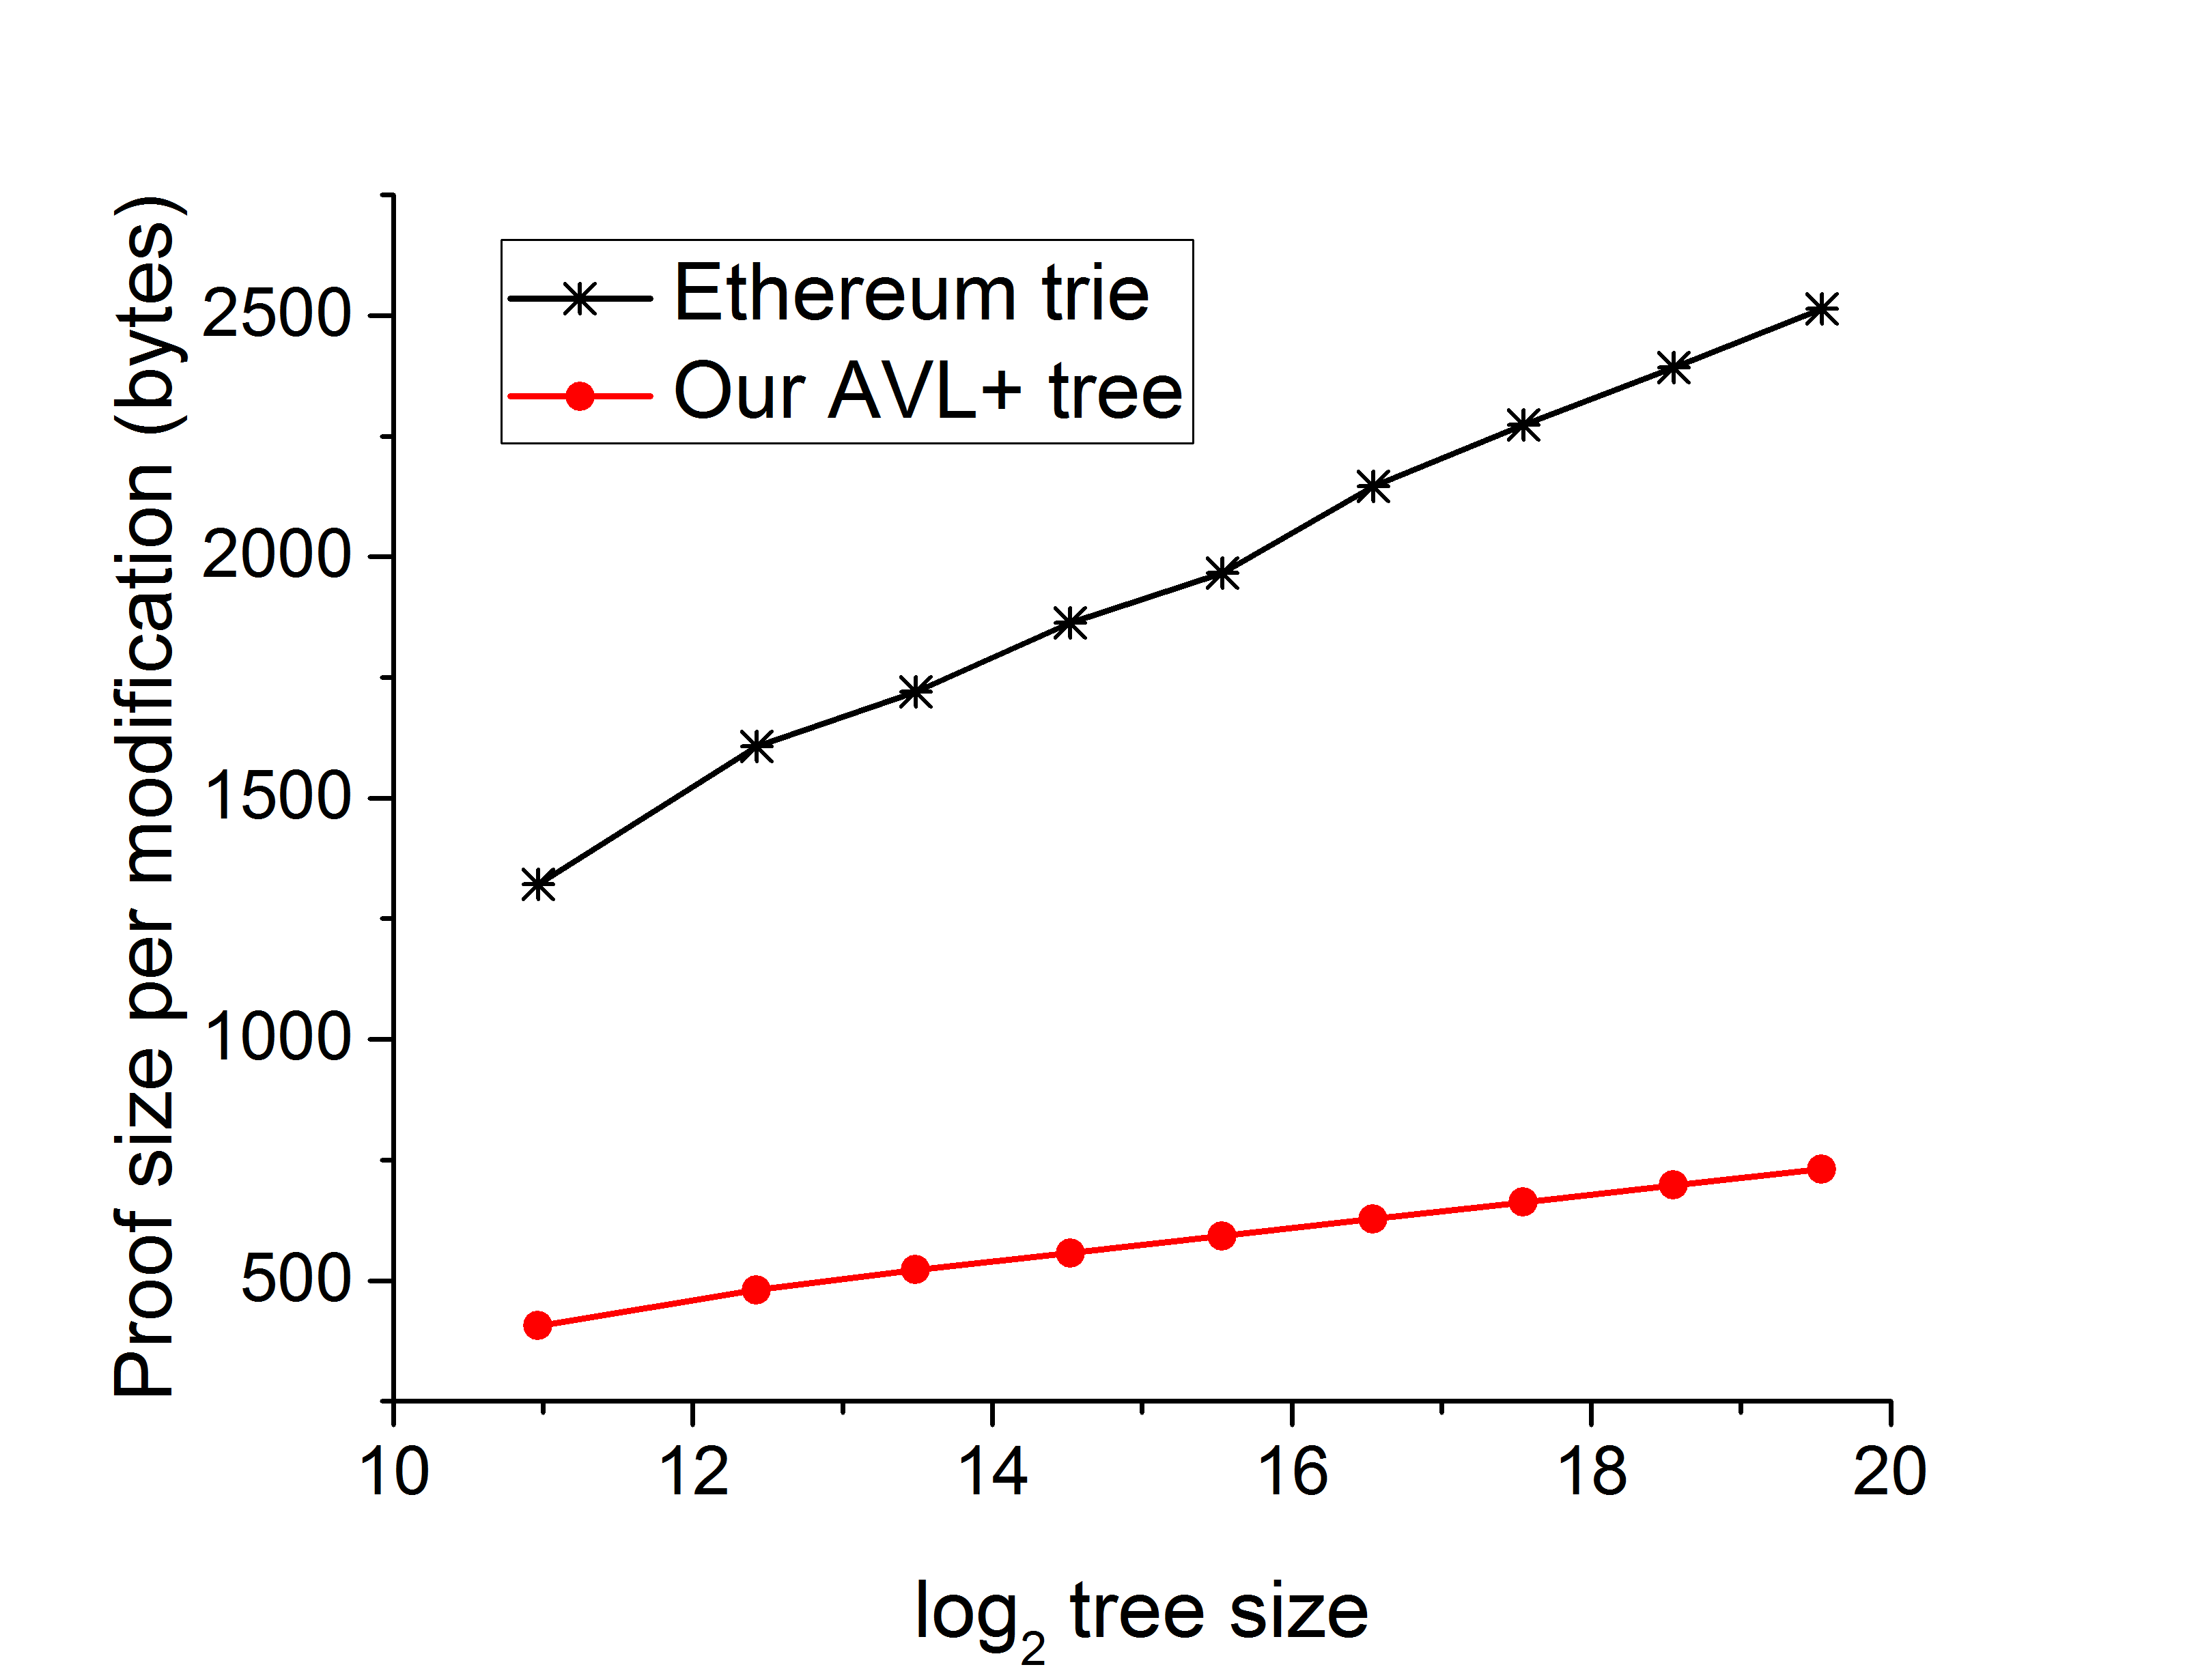
\includegraphics[width=0.5\textwidth]{img/proofSize.png}
    \caption{Proof size comparison with Merkle patricia trie
    \label{fig:proofSize} }
\end{figure}

Finally, proofs for multiple transactions in a single block are compressed together, reducing their total length
by approximately an additional factor of 2:

\begin{figure}[H]
    \centering
    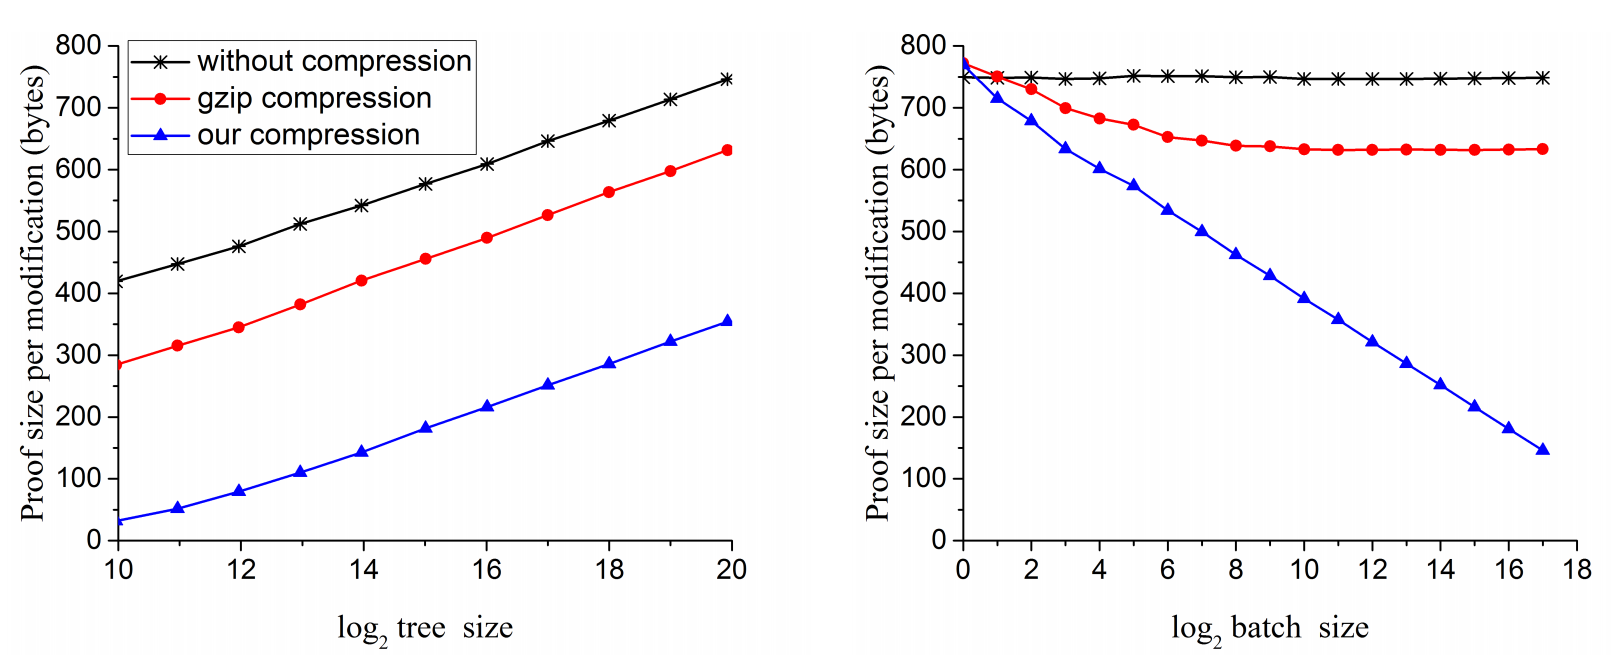
\includegraphics[width=\textwidth]{img/compression.png}
    \caption{Left: proof size per modification for 2000 transactions, as a function of starting tree size n.
    Right: proof size per modification for a tree with n = 1 000 000 keys, as a function of batch size B.
    In both cases, half of the modifications were inserts of new (key, value) pairs and half were changes
    of values for existing keys.
    \label{fig:compression} }
\end{figure}

Thus, Ergo state provide an efficient and secure way to prove existence or non-existence of certain elements in
it, as well as proofs for tree modifications.
These tree operations are supported by Ergo smart contract language, providing a way to implement complicated
contracts like discussed in~\ref{sec:contractual}







    \section{Survivability}
\label{sec:survivability}

% well-tested solutions
% voting
% soft-forkability
% storage rent
% light clients (Пробелмы пользователей без легких клиентов, Дайджест узлы, nipopow/flight clients)

Being a platform for contractual money, Ergo should also support long-term contracts for a
period of a person's life.
While even young project are experiencing issues with performance degradation and
adaptability to external conditions, leading to a situation when a decentralized cryptocurrency
depends on a small group of developers, that should provide a hard-fork, otherwise the cryptocurrency
won't survive.

The first common issue is that in pursuit of popularity blockchain developers implement ad-hoc
solutions without proper preliminary research and testing.
Such solutions inevitably lead to bugs, and regardless of whether they were exploited or not
to bug fixes in a centralized manner, that makes the network even less secure.
Ergo approach here is to use stable well-tested solutions, even if that leads to slower
short-term innovation applicability.
Most of Ergo solutions are formalized in scientific papers, presented at peer-reviewed conferences
and are widely discussed in the community.

In particular, Ergo avoid solutions that may be useful for now, but will lead to performance degradation
over time while also preventing some known performance problems of the blockchain technology.
As far as Ergo is a PoW blockchain, it easily allows extracting a small header from the block content.
Simple header allows to validate the work done, while headers chain is enough to select the best chain
and synchronize the network.
Headers chain is much smaller than the full one, however it still growths linearly with time.
Hopefully, modern researches of light clients~\cite{nipopows, flight clients} provide a way to
synchronize the network by downloading only a small subset of headers, unlocking the ability to
use the network without any trust from low-end hardware like smartphones.
In addition, Ergo uses authenticated state\cite{???} and for any transaction included,
a client may download a proof of its correctness.
Thus, regardless of the blockchain size, a regular user with a
smart-phone can join the network and start using Ergo with the same security
guarantees as a full node.

Although support of light clients solves problems of Ergo users, it does not solve problems
of Ergo miners, that still should keep the whole state of the network to efficiently validate
transactions.
In existing blockchain systems, users can put arbitrary data to this state forever,
creating a lot of dust in it and increasing its size over time~\cite{bitcoin utxo dust}.
This leads to serious security issues, as far as when state size does not fit in memory,
an adversary may generate transactions that require access to random parts of this state
leading to DoS attack like an attack to the Ethereum network in 2016~\cite{??}.
To prevent this, Ergo uses economic solution, analyzed in~\cite{chepurnoy2018systematic}: if an
output remains in the state for 4 years without being moved, a miner may charge a small fee for every
byte kept in the state.
This idea is similar to regular cloud storage services, however, it is new for
cryptocurrencies and has several important consequences.
First, Ergo mining will always be stable, unlike Bitcoin and other PoW currencies, in which mining may become unstable after the
initial emission~\cite{carlsten2016instability}.
Second, state size growth becomes controllable and predictable, reducing hardware requirements for Ergo miners.
Third, by collecting a storage fee from outdated boxes, miners return coins to circulation, preventing a steady decrease
of circulating supply due to lost keys~\cite{wsj2018}.
All these effects should support Ergo long-term survivability, both technically and economically.

Another important aspect of survivability is that the environment changes and a blockchain should
adapt to changing hardware infrastructure, appearing ideas that may improve security or
scalability, arising use-cases and so on.
If all the rules are fixed without any ability to change them in a decentralized manner, even
simple constant change may lead to huge debates and community split, e.g. discussion of a block
size limit in Bitcoin led to the network split into several independent coins.

In contrast, Ergo protocol is self-amendable and is able to adapt to the changing environment.
In Ergo parameters like block size can be changed on-the-fly via miners voting.
At the beginning of a 1024 blocks length voting epoch miner is proposing changes~(up to 2 parameters,
e.g. to increase block size and to decrease storage fee factor) and during the rest of epoch miners
vote, whether to approve these changes or not.
If the majority of votes within an epoch are supporting some~(or both) of these changes, a new value of the
parameter should be written into the extension section of the first block of the next epoch and the
network starts to use this update parameter value during block mining and validation.

To absorb more fundamental changes, Ergo is following the approach of soft-forkability, that
allows to change protocol significantly but keeping old nodes operating.
At the beginning of an epoch, miner can also propose to vote for a fundamental change~(e.g.~to
add new instruction to ErgoScript), describing affected validation rules.
Voting for such breaking changes continues for 32768 blocks and requires at least $90\%$ of
"Yes" votes to be accepted.
Once being accepted, 32768 blocks length activation period started to give time to outdated
nodes to update their software version, and after that changes are activated.
If a node is still not updated after the activation period, it skips the specified checks,
but continues to validate all the known rules.
List of previous soft-fork changes is record into the extension to allow light nodes of
any software version to join the network and read validation rules, it should not check.


    \section{Ergo's Native Token}
\label{sec:currency}

Ergo platform has its native token, which is
called \Erg{} and is divisible to up to $10^9$ smallest units, \nanoErg{}s~(a \nanoErg{} is one billionth of an Erg).
\Erg{}s are important for Ergo platform stability and security by several reasons discussed below.

During the initial phase of Ergo's life, miners will receive the reward in \Erg{}s
according to a predefined and hard-coded token emission schedule~(see~\ref{sec:emission} for more details).
These coins will incentivize miners to participate in the Ergo network, securing it from hashrate-based attacks
like the known 51\% attack~\cite{reorgAttack}.

\Erg{} emission will be finished within just eight years, and after that miners will only receive \Erg{}s from
fees.
Although, adjustable over time through miner on-chain voting, Ergo block size and maximum block computational
cost at any given point in time will be limited,
and thus miners are enforced to
choose only a subset of transactions from mempool during times of high load.
Fees will help miners to sort the transactions, preventing spam attacks while allowing miners
to include transactions from honest users in blocks.

Besides network and computation resources, a transaction utilizes storage by increasing state size.
In existing cryptocurrencies, an element of the state, being  a UTXO  in  UTXO-based  blockchains,  called  a box
in  Ergo, once created lives possibly forever without any compensation to miners and some users who must keep this state
in high-cost random-access memory. This leads to a misalignment of incentives and continuously increasing state size.
In contrast, Ergo has a storage rent component that periodically charges users Erg for every byte
included in the state.
This storage rent is making the system more stable by limiting state size or insuring proper compensation for larger
state size, returning lost coins into
circulation and providing an additional stable and predictable reward to miners.

Thus, being a platform for contractual money, Ergo is suitable to build applications and monetary systems
on top of it.
However, participating in such systems would require using the Ergo native token, Erg, as well in order to pay
storage rent and transaction fees which will provide miners strong ongoing incentives to secure the network with
adequate hash power. Users, for their part, will be highly incentivized to purchase, use and save Ergs if they
find applications for Ergo to be of high value.

\subsection{Emission}
\label{sec:emission}


All \Erg{} tokens that will ever circulate in the system are presented in the initial state, which consists of 3 boxes:

\begin{itemize}
    \item{\em No Premine Proof.} This box contains exactly one~\Erg{} and is protected by a script that prevents it from being spent by anyone.
    Thus, it is a long-lived box that will stay in the system until the storage-rent component
    destroys it.
    Its main purpose is to prove that \Ergo{} mining was not started privately by anyone before
    the declared launch date.
    To achieve this, additional registers of this box contain the latest headlines from the media (The Guardian, Vedomosti, Xinhua), as well as the latest block identifiers from Bitcoin and Ethereum.
    Thus, \Ergo{} mining could not have started before certain events in the real world and the cryptocurrency space.

    \item{\em Treasury.} This box contains 4,330,791.5 \Erg{}s that will be used to fund \Ergo{}
    development.
    Its protecting script~\cite{scriptTreasury} consists of two parts.

    First, it ensures that only a predefined portion of the box value is unlocked.
    During blocks 1-525,599 (2 years) 7.5 \Erg{}s will be released every block. Then during blocks 525,600-590,399 (3 months) 4.5 \Erg{}s will be released every block. Finally,
    during blocks 590,400-655,199 (3 months) 1.5 \Erg{}s will be released every block.
    This rule ensures the presence of funds for \Ergo{} development for 2.5 years and, at any moment of time,
    rewards do not exceed 10\% of the total number of coins in circulation.

    Second, it has custom protection from unexpected spending.
    Initially, it requires the spending transaction to be signed by at least 2 of 3 secret keys that are under control of the initial team members. When they spend the box, they are free to
    change this part of the script as they wish, for example by adding new members to protect foundation
    funds.

    During the first year, these funds will be used to cover the pre-issued EFYT token%~\cite{our website with swap }
. After that, they will be distributed in a decentralized manner via a community voting system that is under development.


    \item{\em Miners Reward.} This box contains 93,409,132 \Erg{}s that will be collected by block miners
    as a reward for their work.
    Its protecting script~\cite{scriptEmission} requires the spending transaction to have exactly two outputs with the following properties:

    \begin{itemize}
    \item{} The first output should be protected by the same script and the number of \Erg{}s in it should
    equal to the remaining miners' reward.
    During blocks 1 - 655,199, a miner will be able to collect 67.5 \Erg{}s from this box. During blocks 655,200 - 719,999 (3 months), a miner will be able to collect 66 \Erg{}s, and after that, the block reward will be reduced by 3 \Erg{}s every 64,800 blocks (3 months) until it reaches zero at block 2,080,800.

    \item{} The second output should contain the remaining coins and should be protected by the following condition:
    it can be spent by a miner that solved the block's PoW puzzle and not earlier than 720 blocks after the current block.
    \end{itemize}

\end{itemize}

All of these rules result in the following curve denoting the number of coins in circulation with time:

\begin{figure}[H]
    \centering
    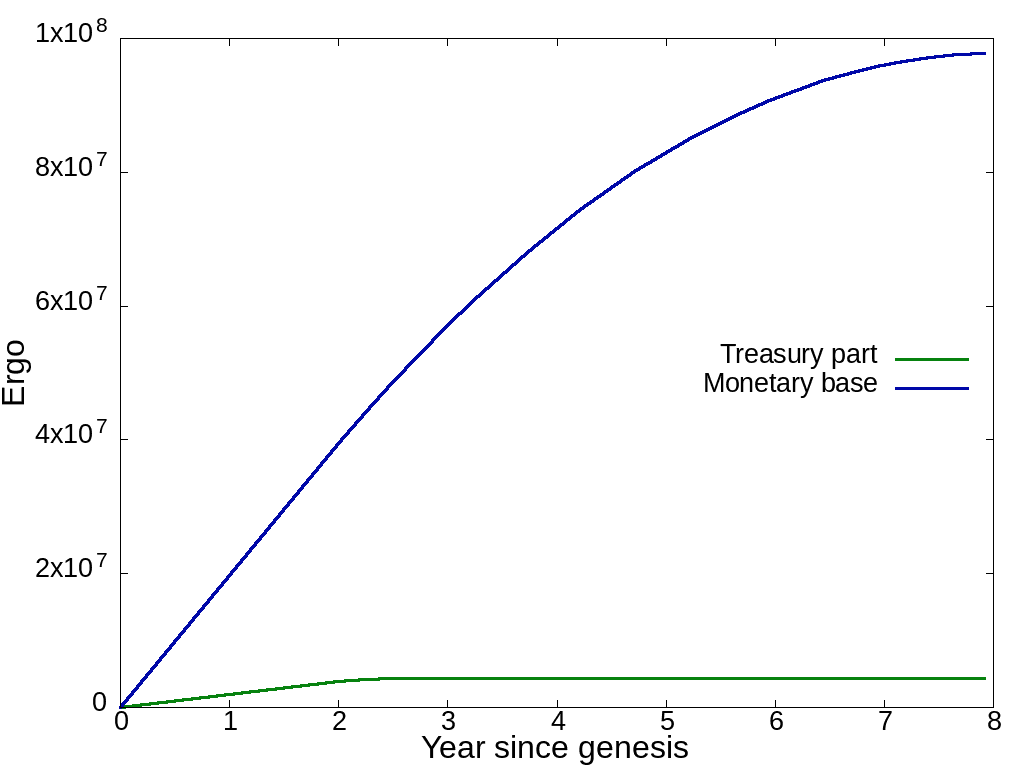
\includegraphics[width=\textwidth]{img/emission.png}
    \caption{Ergo emission curve
    \label{fig:emission} }
\end{figure}


    \section{Contractual Money}
    \label{sec:contractual}

    %   пишет Саша

    %   ценность нашего токена, и филосовские размышления о данном типе экономики
    %   практические удобные и эффективные контракты для денег
    %   Описать про UTXO модель, почему мы ее выбрали
    %   Скрипт - доступ к стейту, доступ к блокчейну, цепочки (тут можно сослаться на Эфир, ибо там написано что в UTXO это невозможно), сигма протоколы
    %   token system - токены на базовом уровне, сильно упрощают протоколы вида "token threshold", позволяют разграничить потоки
    %   ? Анонимность и пример контракта миксинга
    %   Примеры 1-2 контракта, который иллюстрируют несколько основных преимуществ эрго


\subsection{Ergo Token Value}
 \label{sec:ergo-value}

 In this section we are going to provide some reflections on nature of the native Ergo token. For starters, we note that
 any currency is about three main functions: medium of exchange, unit of account, and store of value.

 Bitcoin, being historically the first digital scarce asset, is a perfect as store-of-value. It is even better than
 gold under certain assumptions~(such as SHA-256 hash function not being broken, and majority of miners are not willing
 to destroy the Bitcoin), as emission is limited and known in advance. However, being perfect store-of-value also means
 to be not so good as medium-of-exchange. In particular, if one knows that Bitcoin is indeed the best tool to store
 value in the long term, he would use fiat whenever possible in order to collect more bitcoins.

 On the other hand, Ethereum is not just a currency, but an utility token used to pay for computations over the
 "decentralized world computer" (or "fully replicated programmable calculator"). However, Ethereum is not good as
 store-of-value, as emission in endless, and, historically, can be changed easily by the community core along with
 critical system assumptions.

 Ergo combines best from these two top blockchains. Emission is predefined and limited, more, it will be finished within
 just 10 years. The system assumptions are set in stone with precisely defined {\em social contract}. \knote{link}. Also,
 Ergo is a utility token used to pay for storage rent. This storage rent is making system more stable. Last, Ergo is
 suitable to build monetary systems on top of it with properties different from Ergo native token itself. However,
 participating in such systems would require to use Ergo native token as well in order to pay storage rent.

\subsection{UTXO vs Accounts}
 \label{sec:utxo}

 To check a new transaction, a cryptocurrency client is not using the ledger (all the transactions happened before the
 transaction), rather, it is using ledger state snapshot got from the history. In Bitcoin Core reference implementation,
 this snapshot is about active one-time coins, and a transaction is destroying some coins and also creating new ones.
 In Ethereum, the snapshot is about long-living accounts, where an account is controlled whether by a human or
 executable code; a transaction then is modifying monetary balance and internal memory of some accounts. Also, the
 representation of the snapshot in Ethereum~(unlike Bitcoin) is fixed by the protocol, as authenticating digest of the
 snapshot is written into a block header (thus, in order to have full security guarantees, a client needs to build
 the same snapshot as a miner).

 Ergo is representing the snapshot in form of one-time coins, like Bitcoin. The difference is, in addition to monetary
 value and protecting script, an Ergo coin contains additinal registers with arbitrary data, thus we use term {\em box}
 instead of {\em coin}. Also, like in Ethereum, the ledger snapshot representation~(in form of boxes not destroyed by
 previous transactions) is fixed by the Ergo protocol.

\subsection{The Ergo As The Platform}
 \label{sec:platform}

 In our opinion, 99\% of public blockchain use-cases are about financial applications, even in the presence of a
 general-purpose decentralized world computer, such as Ethefeum Classic. For example, even if an oracle is writing
 non-financial data into a blockchain (such as temperature), this data is usually to be written to be used in a financial
 contract. Another trivial observation we have made, is that many applications are using digital tokens with mechanics
 different from a native token of a blockchain system~(especially application built on top of Ethereum).

 Thus Ergo offers for an application developer in-built tokens~(with minimal functionality per se, in comparison with
 Waves or Nxt), and domain-specific language for box guarding condition which is powerful enough to define rich
 financial applications. Thus Ergo applications are defined in terms of guarding scripts built into boxes also containing
 data possibly involved into execution. We coin the term {\em contractual money} for Ergs and secondary tokens which
 usage is bounded by a contract. In narrow sense, we can distinguish Ergs in existence as ones which could easily
 change their contracts from Ergs which are bounded by contracts in the sense that a box with contractual Ergs is
 demanding from a spending transaction to create boxes with some properties. We will refer to the former as to ordinary
 (or cleared, or free) Ergs, and to the latter as to the contractual Ergs. Similarly, we can define contractual tokens.

 For example, if a box is protected just by a public key~(so providing a signature against a spending transaction is
 enough in order to destroy the box), a public key owner may create an arbitrary box replacing the one being protected
 by the public key, thus the Ergs within the box are free to change the contract. In contrast, imagine a box "B" which
 is protected by combination of a public key and also condition which demands a spending transaction to create an output
 box which guarding script hash is equal to "rBMUEMuPQUx3GzgFZSsHmLMBouLabNZ4HcERm4N" (in Base58 encoding), and Ergs
 value of the output should equal to the value of the original box. In this case box value is bounded by the contract,
 thus Ergs in the box are contractual Ergs.

\subsection{Difference From Bitcoin}

 While in Bitcoin a transaction output~(a digital coin) is protected by a program in stack-based language, in Ergo a
 box is protected by a logic formula which combines predicates over a context and cryptographic statements provable
 via zero-knowledge protocols with AND, OR, and k-out-of-n connectives. The formula is represented as a typed direct
 acyclic graph, which serialized form is written in a box. To destroy a box, a spending transaction needs to provide
 arguments, including zero-knowledge proofs, which are enough to satisfy the formula.

 However, in most cases a developer is unlikely to develop box contracts in terms of graphs. Instead, he would likely
 using a high-level language, and we provide one called ErgoScript. Writing scripts in this language is easy, for
 example, for a one-out-of-two signature, protecting script would be ${pk_1 \&\& pk_2}$, which means "prove knowledge of
 a secret key corresponding to the public key $pk_1$, or knowledge of a secret key corresponding to $pk_2$". We have
 two separate documents which are helping to develop contracts with ErgoScript, the "ErgoScript Tutorial"~\cite{}
 and "Advanced ErgoScript Tutorial"~\cite{}. Thus below we are not going to dive into developing contracts with
 ErgoScript, rather, we are going to provide a couple of motivation examples.

\subsection{Data Inputs}
 \label{sec:data-inputs}

 A box could be not only destroyed by a transaction, but is also could be only read, in the latter case we refer to the
 box as to {\em data input} of the transaction. Thus a transaction is getting two box sets as its arguments, inputs and
 data inputs, and produces a box set named {\em outputs}. Data inputs are useful for oracle applications and interacting
 contracts.

\subsection{Custom tokens}
 \label{sec:custom tokens}

 A transaction can carry many tokens, if only estimated complexity for processing them is not exceeding a limit. A
 transaction is also able to issue a token, but only one, and with a unique~(and cryptographically strong against
 finding a collision) identifier, which is equal to identifier of a first~(spendable) input box of the transaction.
 The amount of the tokens issued could be any number within the [1, 9223372036854775807] range. For the tokens, the weak
 preservation rule is defined, which is demanding total amount for a token in transaction outputs should be no more
 than total amount for the token in transaction inputs~(thus some amount of token could be burnt). In contrast, for Ergs
 a preservation rule is strong, thus total Ergs amount for inputs should be equal to total Ergs amount for outputs.

\subsection{An Oracle Example}
 \label{sec:platform}

 Equipped with custom tokens and data inputs, we can develop a simple oracle example, also showing on the way some
 design patterns for Ergo contracts. In the example, Alice and Bob are putting money into a box, which is spendable by
 Alice if temperature is more than 15 degrees, and is spendable by Bob otherwise. To deliver temperature into the
 blockchain a trusted oracle is needed.

 In opposite to Ethereum with its long-lived accounts, where trusted oracle identifier is usually known in advance,
 delivering data with one-time boxes is more tricky. For starters, a box which is protected by an oracle's key could
 not be trusted, as anyone can create such a box. It is possible to include a signed data into a box, and check the
 signature in the contract using the data, we have such an example, but this example is quite involved. With custom
 tokens, however, a solution is pretty simple.

 In the first place, a token identifying the oracle should be issued. In the simplest case, amount for the token could
 be equal to one. Then the oracle is creating a box which contains the token and also temperature, for example, in the
 register number four~($R4$). In order to update temperature, an oracle is destroying the outpdate box and creating a
 new one with updated temperature.

 Then, like in Ethereum, Alice and Bob usually know oracle's token identifier in advance. With this knowledge, they
 can jointly create a box which requires first data input (which is read-only) to contain the oracle's token. The
 contract is extracting temperature from the data input and decides who is getting the payout. The code is as simple as


 \begin{algorithm}[H]
    \caption{Oracle Contract Example}
    \label{alg:oracle}
    \begin{algorithmic}[1]
        \State val dataInput = CONTEXT.dataInputs(0)
        \State val inReg = dataInput.R4[Long].get
        \State val inToken = dataInput.tokens(0).\_1 == tokenId
        \State val okContractLogic = (inReg $>$ 15L \&\& pkA) $||$ (inReg $<=$ 15L \&\& pkB)
        \State inToken \&\& okContractLogic
    \end{algorithmic}
 \end{algorithm}

\subsection{A Mixing Example}
 \label{sec:platform}

 Privacy is important for a digital currency, but implementing it in a protocol could be costly or require a trusted
 setup. Thus we are looking for ways to do coin mixing via cheap enough applications. As a first step towards that, we
 offer an application for non-interactive coin mixing, which is working in the following case:
 \begin{enumerate}
    \item{} Alice creates a box which demands any Bob's coin to satisfy certain conditions in order to be mixed with
    the coin of Alice. After that, Alice only listens to the blockchain, no any interaction with Bob is needed.
    \item{} Bob is creating a box and then a spending transaction which has boxes of Alice and Bob as inputs,
     and creates two outputs with the same script, but both Alice and Bob may spend only one box out of the two.
     An external observer can coin spent by whom, as output boxes are indistinguishable.
 \end{enumerate}

 For simplicity, we are not considering fees in the example.

 \begin{algorithm}[H]
    \caption{Mixing Transaction Output Script}
    \label{alg:oracle}
    \begin{algorithmic}[1]
        \State val c1 = OUTPUTS(0).R4[GroupElement].get
        \State val c2 = OUTPUTS(0).R5[GroupElement].get
        \State
        \State OUTPUTS.size == 2 \&\&
        \State OUTPUTS(0).value == SELF.value \&\&
        \State OUTPUTS(1).value == SELF.value \&\&
        \State blake2b256(OUTPUTS(0).propositionBytes) == fullMixScriptHash \&\&
        \State blake2b256(OUTPUTS(1).propositionBytes) == fullMixScriptHash \&\&
        \State OUTPUTS(1).R4[GroupElement].get == c2 \&\&
        \State OUTPUTS(1).R5[GroupElement].get == c1 \&\& \{
        \State\hspace{\algorithmicindent}  proveDHTuple(g, gX, c1, c2) $||$
        \State\hspace{\algorithmicindent}  proveDHTuple(g, gX, c2, c1)
        \State \}
    \end{algorithmic}
 \end{algorithm}

 \begin{algorithm}[H]
    \caption{Mixing Transaction Output Script}
    \label{alg:oracle}
    \begin{algorithmic}[1]
        \State val c1 = SELF.R4[GroupElement].get
        \State val c2 = SELF.R5[GroupElement].get
        \State proveDlog(c2) $||$            // either c2 is $g^y$
        \State proveDHTuple(g, c1, gX, c2) // or c2 is $u^y = g^{x \cdot y}$
    \end{algorithmic}
 \end{algorithm}


\subsection{The Local Exchange Trading System}
 \label{sec:platform}

 Here we briefly overview a local exchange trading system implementation. In such system, a member of a community may
 issue community currency via personal debt. For example, if Alice with zero balance is buying something for 5
 community tokens from Bob, which balance is about zero as well, her balance after the trade would be -5 tokens, and
 Bob's balance would be 5 tokens. Then Bob could buy something for 5 tokens, for example, from Carol. Usually, in such
 systems there is a limit for negative balance.

 As digital community could be vulnerable to sybil attacks, thus some mechanism is needed in order to prevent creation
 of sybils creating debts. We consider two solutions, namely, a committee of trusted managers approving new members of
 the community, or securitуy deposits made in Ergs. For simplicity, we consider the approach with the committee here.

 This example is about two interacting contracts then. In the first place, a management script is about maintaining a
 community members list, and a new member could be added if management condition (e.g. threshold signature from a
 committee) satisfied. In the second

\subsection{More Examples}




    \bibliography{references}

\end{document}
